\section{Disturbed closed orbits}\label{sec:2.10}

Until now I have considered the trajectories of electrons in a prescribed guide field. I wish next to consider the following question: Suppose we have analyzed the electron trajectories for this prescribed field; how will the trajectories be different if there are small deviations of the fields from the assumed prescription? In our linear approximation, the prescribed - or \emph{nominal} - guide field was specified by giving its value on the ideal orbit and its radial derivative. See Section \ref{sec:2.3}. Also, it was assumed that the field at the ideal orbit was everywhere vertical. I wish now to inquire about the effects of small deviations from the nominal field. If the vertical magnetic field at the ideal orbit differs
 from its nominal value, or if there is some small horizontal field, the lateral accelerations
will be different from what is necessary to keep an electron on the design orbit. The deviations
 of the field at the design orbit will be called \emph{field errors}. Changes in the fields which cause the focusing functions $K_x$ and $K_y$ to differ from their nominal values will, for convenience, be called \emph{gradient errors}\footnote{Although field errors will, through the term $G^2$ in Eq. \eqref{eq:2.17} also change $K_x$, such effects are not usually important.}.\\
When there are field errors, the design orbit is no longer a possible trajectory. If the errors
 are small, however, there will be another closed curve which is a possible orbit for an electron
 of the nominal energy. I shall call this trajectory the \emph{disturbed closed orbit}. The general trajectory will execute betatron oscillations with respect to this disturbed closed orbit. And the form of the betatron oscillations will be determined by the modified focussing function. That is, if we continue to let x represent the displacement from the original design orbit, we may write
\begin{align}\label{eq:2.83}
	x = x_c + x_\beta,
\end{align}
where $x_c$ is the displacement of the disturbed closed orbit from the ideal one, and $x_\beta$ is the “free” betatron oscillation about the disturbed closed orbit.\\
If the closed orbit displacements are small, our assumed linearity of the field variations means that the betatron oscillations are the same with respect to the disturbed closed orbit as they would be with respect to the design orbit. We may therefore, consider separately the distortions
 of the closed orbit caused by field errors and the disturbances to the betatron oscillations
 caused by gradient errors. And we may interpret Eq. \eqref{eq:2.83} as a superposition of the closed orbit distortion $x_c$ and a free betatron oscillation $x_\beta$ that is calculated with respect to the design orbit by the methods we have been using until now.\\
Let’s look first at the effect of the field errors. Suppose we begin by considering the effect of a field error which exists only in a small azimuthal interval $\Delta s$, which we may as well place at $s = 0$. In passing through $\Delta s$ the displacement $x$ is unchanged, but the slope $x'$ change by the amount
\begin{align*}
	\Delta x' = - \dfrac{ec\delta B}{E_0}\Delta s,
\end{align*}
where $\delta B$ is the deviation of the magnetic field from its nominal value. For the vertical
 motion we would have the same form if $\delta B$ were identified as the total radial field at the design orbit (with a suitably chosen sign). In keeping with the definition of Eq. \eqref{eq:2.3} we set $ec \delta B/E_0 = \delta G$ with a suitable subscript $x$ or $y$ implied when we are considering the radial or vertical motion. We may, as before, consider only a generic $x$-motion with the understanding that all the results apply equally to $x$-motion
 or to $y$-motion when all identifying subscripts are restored. We write, then the effect of the field error in $\Delta s$ as
\begin{align}\label{eq:2.84}
	\Delta x' = -\delta G \Delta s.
\end{align}
The field error at $s$ adds to $x'' = \Delta x'/\Delta s$ a term $\delta G$; and is, therefore, equivalent to adding a driving force $\delta G(s)$ to the equation of motion. We get the complete
equation of motion for $x_c$ by adding this new force term to the usual equation for $x$, Eq. \eqref{eq:2.31}:
\begin{align}\label{eq:2.85}
	x'' = -K(s)x -\delta G(s).
\end{align}
The displacement $x_c$ of the disturbed closed orbit is the solution of this equation
that is single valued at each physical azimuth.\\
We may make an estimate of the effect of a localized field error at $s = 0$ by using the approximate harmonic form of the betatron motion described in Section \ref{sec:2.9}. Think for the moment of an electron that is traveling along the design orbit - so that its slope $x'$ is zero. When it arrives at $s = 0$ its slope is suddenly changed to $\Delta x'$. See Fig. \ref{fig:fig21}. After $s = 0$ there is no field error (for one full revolution) so the electron begins to oscillate about the ideal orbit with the amplitude
\begin{align}\label{eq:2.86}
	b = \lambda \Delta x' = -\lambda \delta G \Delta s.
\end{align}
We may expect the closed orbit displacement $x_c$ to be of the same order of magnitude.
\begin{figure}[!htb]
	\centering
	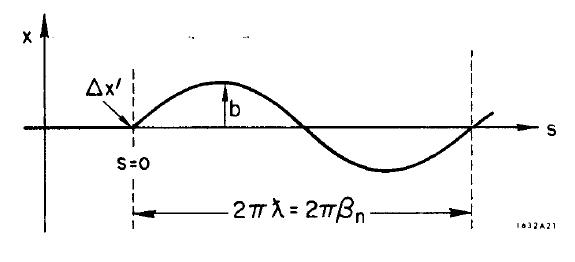
\includegraphics[width=0.8\linewidth]{./Figuras/fig21.jpeg}
	\caption{Effect of a localized field error.}
	\label{fig:fig21}
\end{figure}
To make a proper calculation of $x_c$, we should use the correct pseudo-harmonic free oscillation, and remember also that the displaced closed orbit is defined as that particular
 trajectory which closes on itself after one revolution. In other words $x_c$ must be single valued at each physical azimuth $s$, namely $x_c(s + L) = x_c(s)$. In particular,
 \begin{align}
	x_c(L) = x_c(0);
\end{align}
and by Eq. \eqref{eq:2.84},
\begin{align}
	x_c'(L) - \delta G \Delta s = x_c'(0).
\end{align}
But between $s = 0$ and $s = L$ there are no field errors, so $x_c$ is just a free oscillation about the ideal orbit. See Fig. \ref{fig:fig22}. That is, $x_c$ must be given by Eq. \eqref{eq:2.46}:
\begin{figure}[!htb]
	\centering
	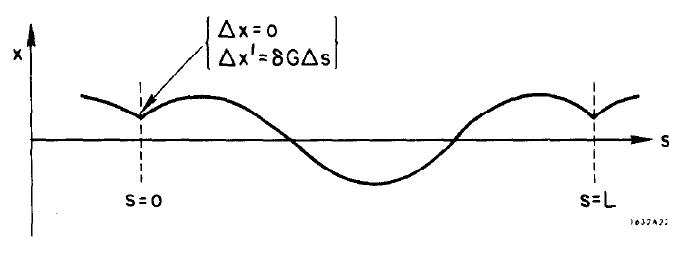
\includegraphics[width=0.8\linewidth]{./Figuras/fig22.jpeg}
	\caption{The disturbed closed orbit for a field error at $s = 0$.}
	\label{fig:fig22}
\end{figure}
Using Eq. \eqref{eq:2.52} for $x_c'(s)$ - everywhere but at $s = 0$ - you may verify that the
appropriate values of $a$ and $\vartheta$ are\footnote{The phase constant $\vartheta$ is, of course, only defined within an integral multiple of $2\pi$.}
\begin{align}
	a &= -\dfrac{\delta G \Delta s \sqrt{\beta(0)}}{2 \sin \pi \nu},\\
    \vartheta &= \pi\nu.
\end{align}

\begin{proof}
From Eq. \eqref{eq:2.52} we obtain
\begin{align*}
x_c'(s) =\dfrac{\beta'(s)x}{2\beta(s)} - \dfrac{a}{\sqrt{\beta(s)}}\sin\left(\varphi(s) - \vartheta\right).
\end{align*}
Since $x$ and $\beta$ are periodic, i.e., $x(0)=x(L)$ and $\beta(0) = \beta(L)$, $\varphi(L) - \varphi(0) = 2 \pi \nu$, by definition, and $\varphi(s=0)=0$, we use $\Delta x' =  \delta G \Delta s$,
to get the following expression
\begin{align*}
\dfrac{a}{\sqrt{\beta(0)}}\left[\sin(2\pi \nu - \vartheta) - \sin(-\vartheta)\right] = \delta G \Delta s.
\end{align*}
The terms between squared brackets can be simplified as follows
\begin{align*}
\sin(2\pi \nu - \vartheta) - \sin(-\vartheta) &= \sin(2\pi \nu)\cos\vartheta - \cos(2\pi \nu)\sin \vartheta + \sin \vartheta\\
                                         &= 2\sin(\pi \nu)\cos(\pi \nu)\cos\vartheta + \left(1-\cos(2\pi \nu)\right)\sin\vartheta\\
                                           &= 2\sin(\pi \nu)\cos(\pi \nu)\cos\vartheta + 2\sin^2(\pi \nu)\sin\vartheta\\
                                           &= 2\sin(\pi\nu)\left[\cos(\pi\nu)\cos\vartheta + \sin(\pi\nu)\cos\vartheta\right] \\
                                           &=  2\sin(\pi\nu)\cos(\pi\nu - \vartheta).
\end{align*}
Therefore
\begin{align*}
2\sin(\pi\nu)\cos(\pi\nu - \vartheta)\dfrac{a}{\sqrt{\beta(0)}} = -\delta G \Delta s,
\end{align*}
and we see that the preceding expression holds if $a = -\dfrac{\delta G \Delta s \sqrt{\beta(0)}}{2 \sin \pi \nu}$ and $\vartheta = \pi \nu$.
\end{proof}

The displacement of the disturbed closed orbit is then
\begin{align}\label{eq:2.92}
	x_c(s) = -\dfrac{\delta G \Delta s \sqrt{\beta(0)}}{2 \sin\pi\nu}\sqrt{\beta(s)}\cos\{\varphi(s)-\pi\nu\}.
\end{align}
The form of the amplitude invariant $a$ displays the two most interesting features of the disturbed closed orbit. Notice first, that the displacement of the closed orbit is everywhere
 proportional to the ``strength'' $\delta G \Delta s$ of the field error, \emph{and to the root of} $\beta(0)$, \emph{the magnitude of the betatron function at the location of the perturbation}. You see why one may consider that $\beta(s)$ or more precisely $\zeta(s) = \sqrt{\beta(s)}$ - is a measure of the ``sensitivity'' to disturbances.\\
Second, notice that the denominator of $a$ goes toward zero, and $x_c$ becomes, therefore, very large whenever the tune $\nu$ approaches an integer. It is this behavior which was referred
 to earlier as an integral resonance which must be avoided in choosing the operating point $(\nu_x, \nu_y)$.\\
Notice that the displacement of the closed orbit at the location of the error has a particularly
 simple form. You just set $s = 0$ in Eq. \eqref{eq:2.92}, or generalizing to an error $\delta G$ located in $\Delta s$ at an arbitrary azimuth, say $s_1$, you get
 \begin{align}
	x_c(s_1) = -\delta G \Delta s \dfrac{\beta{(s_1)}}{2 \tan\pi\nu}.
\end{align}
The displacement is now proportional to the first power of $\beta$, but the same resonance
dependence on $\nu$ is evident in the tangent factor. Notice also that except for the resonant denominator, this result agrees with the estimate given in Eq. \eqref{eq:2.86}.
We may also generalize Eq. \eqref{eq:2.92} to give the closed orbit distortion for an
arbitrary distribution $\delta G(s)$ of field errors around the ring. At each azimuth $s$ the closed orbit displacements caused by the errors at all other azimuths will add. For an error
 at $\bar{s} \in [0,L[$ we should replace $s = 0$ by $\bar{s}$ in Eq. \eqref{eq:2.92} - and at the same time replace $\varphi(s)$ by $\varphi(s) - \varphi(\bar{s})$, obtaining
\begin{align}\label{eq:dist_closed_orb}
x_c(s) = -\dfrac{\sqrt{\beta(\bar{s})\beta(s)}}{2\sin\pi\nu} \cos(\varphi(s)-\varphi(\bar{s})-\pi\nu)\delta G(\bar{s})\Delta\bar{s}.
\end{align}
However, we cannot sum over all $\Delta \bar{s}$ to obtain the total disturbed closed orbit, since each function has a different domain, which is $[\bar{s},\bar{s}+L[$. Note, for example, that Eq.~\eqref{eq:2.92} is valid only for $0 \leq s < L$. In order to extend the domain of the functions such that the intersection of all domains give us $[0,L[$ (the whole ring), it is sufficient to replace $\varphi(s) - \varphi(\bar{s})$, in Eq.~\eqref{eq:dist_closed_orb}, by $|\varphi(s) - \varphi(\bar{s})|$, thus extending the domain to $]\bar{s}-L,\bar{s}+L[$. One can check this by verifying that for $s \in ]\bar{s}-L,\bar{s}[$,
\begin{align*}
	\cos(|\varphi(s) - \varphi(\bar{s})| - \pi\nu) = \cos(\varphi(s+L) - \varphi(\bar{s})-\pi\nu),
\end{align*}
and for $s \in [\bar{s},\bar{s}+L[$,
\begin{align*}
\cos(|\varphi(s) - \varphi(\bar{s})| - \pi\nu) = \cos(\varphi(s) - \varphi(\bar{s}) - \pi\nu)
\end{align*}
Finally, we can add up all contributions, obtaining thus, for $s \in [0,L[$,
\begin{align}\label{eq:2.94}
	\boxed{ x_c(s) = -\dfrac{\sqrt{\beta(s)}}{2\sin\pi\nu} \oint \delta G(\bar{s}) \sqrt{\beta(\bar{s})}\cos\{ |\varphi(s) - \varphi(\bar{s})| - \pi\nu \} d\bar{s} }.
\end{align}
If we have a known field deviation $\delta G(s)$, this equation will (with $\beta(s)$ and $\nu$ taken as their undisturbed values) give us the form of the displaced closed orbit.\\
If the field deviations are true ``errors'' with an unknown statistical distribution, a more complex statistical analysis must be made to arrive at a statistical estimate of $x_c$. I shall not go into that subject here.\\
As mentioned earlier the total displacement from the ideal orbit is the sum of $x_c$ and a free betatron oscillation. In the following sections I shall ignore $x_c$ with the understanding
 that it must always be added in, when one wishes to find the total displacement of a trajectory
 from the design orbit.

 \subsection{Closed orbit correction}

 The orbit correction system in storage rings has Beam Position Monitors (BPMs) and small dipoles magnets, called correctors or steering magnets, that steer the beam depending on orbit distortions measured by the BPMs.

 The orbit distortion in the presence of localized field errors $\delta G(s_j)$ at different positions $s_j$ along the ring is given by:
	\begin{align*}
		u_c(s_i) = \dfrac{\sqrt{\beta_u(s_i)}}{2\sin\pi\nu} \sum_j \delta G({s}_j) \sqrt{\beta_u({s}_j)}\cos\{ |\varphi(s_i) - \varphi({s}_j)| - \pi\nu \} \Delta s_j,
	\end{align*}
	where $u$ may represent the $x$ or $y$ coordinate.  The orbit distortions $\Delta u(s_i)$ can be measured in localized positions $s_i$, where BPMs are installed, and localized dipolar fields $\delta G(s_j)$ (typically called ``kicks'') can be created by the correctors, also in localized positions $s_j$. The above equation can be cast in the form $\Delta u_i = \sum_{j} M_{ij}^{uu} \Delta \theta_{j}^u$ (identifying $\Delta \theta_{j}^u = \delta G(s_j) \Delta s_j$). Therefore, one can define the orbit response matrix, whose elements can be recognized as:
 \begin{align}
 M_{ij}^{uu} = \dfrac{\sqrt{\beta_{u}(s_i)\beta_{u}(s_j)}}{2\sin\left(\pi\nu_{u}\right)}\cos\left( |\varphi_{u}(s_i) - \varphi_{u}(s_j)| - \pi\nu_{u} \right).
 \end{align}

 The orbit distortions measurements and the kick variations can be sorted in vectors as
 \begin{align*}
	 \Delta \vec{u} &= \left(\Delta x_1, \ldots, \Delta x_{\mathrm{N}_{\mathrm{BPM}}}, \Delta y_1, \ldots, \Delta y_{\mathrm{N}_{\mathrm{BPM}}}\right), \\
	 \Delta \vec{\theta} &= \left(\Delta \theta_1^x, \ldots, \Delta \theta_{\mathrm{N}_{\mathrm{CH}}}^x, \Delta \theta_1^y, \ldots, \Delta \theta_{\mathrm{N}_{\mathrm{CV}}}^y\right).
 \end{align*}

 $\mathrm{N}_{\mathrm{BPM}}$ is the number of BPMs, $\mathrm{N}_{\mathrm{CH}}$ is the number of horizontal correctors (CH) and $\mathrm{N}_{\mathrm{CV}}$ is the number of vertical correctors (CV). In this vectorial form, the orbit distortion created by the kicks variation is given by $\Delta \vec{u} = \mathbf{M} \Delta \vec{\theta}$, and the orbit response matrix has dimension $2 \mathrm{N}_{\mathrm{BPM}} \times \left(\mathrm{N}_{\mathrm{CH}} + \mathrm{N}_{\mathrm{CV}}\right)$.

 Suppose that the BPMs measure the orbit distortion $\vec{u}_{\mathrm{d}}$. With the correctors it is possible to produce an orbit variation that minimizes the 2-norm of the residual orbit. From the minimization of $||\vec{u}_{\mathrm{d}} - \mathbf{M}\Delta \vec{\theta}||^2$ with respect to $\Delta\vec{\theta}$, the required kick variations are $\Delta \vec{\theta} = -\mathbf{M}^{-1}\vec{u}_{\mathrm{d}}$. The orbit response matrix may be non-square and in these cases the symbol $\mathbf{M}^{-1}$ must be viewed as a pseudo-inverse. Since the actual problem may be non-linear, the corrections must be calculated and applied iteratively until convergence.

 The pseudo-inverse of $\mathbf{M}$ can be obtained, for example, with the method of Singular Value Decomposition (SVD), with a suitable choice of singular values used in the pseudo-inversion procedure. The SVD-based orbit correction is quite common in storage rings but there are other algorithms also available, depending on the application purpose.
